\documentclass{beamer}
%\documentclass[trans]{beamer}
%\mode<presentation>

\usetheme{default}%Warsaw}
\usecolortheme{seahorse}
\usecolortheme{rose}
%\useinnertheme{circles}
%\setbeamertemplate{headline}{}
%\usefonttheme{serif}
\useoutertheme[subsection=false,footline=none]{miniframes}
\setbeamertemplate{theorems}[numbered]
\usepackage{xmpmulti}
\usepackage{algorithm2e}
\usepackage{tikz}
\usetikzlibrary{arrows,shapes,positioning,snakes,calc,patterns}
\usepackage{pgfplots}
\pgfplotsset{compat=1.5.1}
\usepackage{booktabs,multirow}
\usepackage{fancyvrb}
\usepackage{color}
\usepackage[latin1]{inputenc}



\makeatletter
\def\PY@reset{\let\PY@it=\relax \let\PY@bf=\relax%
    \let\PY@ul=\relax \let\PY@tc=\relax%
    \let\PY@bc=\relax \let\PY@ff=\relax}
\def\PY@tok#1{\csname PY@tok@#1\endcsname}
\def\PY@toks#1+{\ifx\relax#1\empty\else%
    \PY@tok{#1}\expandafter\PY@toks\fi}
\def\PY@do#1{\PY@bc{\PY@tc{\PY@ul{%
    \PY@it{\PY@bf{\PY@ff{#1}}}}}}}
\def\PY#1#2{\PY@reset\PY@toks#1+\relax+\PY@do{#2}}

\expandafter\def\csname PY@tok@gd\endcsname{\def\PY@tc##1{\textcolor[rgb]{0.63,0.00,0.00}{##1}}}
\expandafter\def\csname PY@tok@gu\endcsname{\let\PY@bf=\textbf\def\PY@tc##1{\textcolor[rgb]{0.50,0.00,0.50}{##1}}}
\expandafter\def\csname PY@tok@gt\endcsname{\def\PY@tc##1{\textcolor[rgb]{0.00,0.27,0.87}{##1}}}
\expandafter\def\csname PY@tok@gs\endcsname{\let\PY@bf=\textbf}
\expandafter\def\csname PY@tok@gr\endcsname{\def\PY@tc##1{\textcolor[rgb]{1.00,0.00,0.00}{##1}}}
\expandafter\def\csname PY@tok@cm\endcsname{\let\PY@it=\textit\def\PY@tc##1{\textcolor[rgb]{0.25,0.50,0.50}{##1}}}
\expandafter\def\csname PY@tok@vg\endcsname{\def\PY@tc##1{\textcolor[rgb]{0.10,0.09,0.49}{##1}}}
\expandafter\def\csname PY@tok@m\endcsname{\def\PY@tc##1{\textcolor[rgb]{0.40,0.40,0.40}{##1}}}
\expandafter\def\csname PY@tok@mh\endcsname{\def\PY@tc##1{\textcolor[rgb]{0.40,0.40,0.40}{##1}}}
\expandafter\def\csname PY@tok@go\endcsname{\def\PY@tc##1{\textcolor[rgb]{0.53,0.53,0.53}{##1}}}
\expandafter\def\csname PY@tok@ge\endcsname{\let\PY@it=\textit}
\expandafter\def\csname PY@tok@vc\endcsname{\def\PY@tc##1{\textcolor[rgb]{0.10,0.09,0.49}{##1}}}
\expandafter\def\csname PY@tok@il\endcsname{\def\PY@tc##1{\textcolor[rgb]{0.40,0.40,0.40}{##1}}}
\expandafter\def\csname PY@tok@cs\endcsname{\let\PY@it=\textit\def\PY@tc##1{\textcolor[rgb]{0.25,0.50,0.50}{##1}}}
\expandafter\def\csname PY@tok@cp\endcsname{\def\PY@tc##1{\textcolor[rgb]{0.74,0.48,0.00}{##1}}}
\expandafter\def\csname PY@tok@gi\endcsname{\def\PY@tc##1{\textcolor[rgb]{0.00,0.63,0.00}{##1}}}
\expandafter\def\csname PY@tok@gh\endcsname{\let\PY@bf=\textbf\def\PY@tc##1{\textcolor[rgb]{0.00,0.00,0.50}{##1}}}
\expandafter\def\csname PY@tok@ni\endcsname{\let\PY@bf=\textbf\def\PY@tc##1{\textcolor[rgb]{0.60,0.60,0.60}{##1}}}
\expandafter\def\csname PY@tok@nl\endcsname{\def\PY@tc##1{\textcolor[rgb]{0.63,0.63,0.00}{##1}}}
\expandafter\def\csname PY@tok@nn\endcsname{\let\PY@bf=\textbf\def\PY@tc##1{\textcolor[rgb]{0.00,0.00,1.00}{##1}}}
\expandafter\def\csname PY@tok@no\endcsname{\def\PY@tc##1{\textcolor[rgb]{0.53,0.00,0.00}{##1}}}
\expandafter\def\csname PY@tok@na\endcsname{\def\PY@tc##1{\textcolor[rgb]{0.49,0.56,0.16}{##1}}}
\expandafter\def\csname PY@tok@nb\endcsname{\def\PY@tc##1{\textcolor[rgb]{0.00,0.50,0.00}{##1}}}
\expandafter\def\csname PY@tok@nc\endcsname{\let\PY@bf=\textbf\def\PY@tc##1{\textcolor[rgb]{0.00,0.00,1.00}{##1}}}
\expandafter\def\csname PY@tok@nd\endcsname{\def\PY@tc##1{\textcolor[rgb]{0.67,0.13,1.00}{##1}}}
\expandafter\def\csname PY@tok@ne\endcsname{\let\PY@bf=\textbf\def\PY@tc##1{\textcolor[rgb]{0.82,0.25,0.23}{##1}}}
\expandafter\def\csname PY@tok@nf\endcsname{\def\PY@tc##1{\textcolor[rgb]{0.00,0.00,1.00}{##1}}}
\expandafter\def\csname PY@tok@si\endcsname{\let\PY@bf=\textbf\def\PY@tc##1{\textcolor[rgb]{0.73,0.40,0.53}{##1}}}
\expandafter\def\csname PY@tok@s2\endcsname{\def\PY@tc##1{\textcolor[rgb]{0.73,0.13,0.13}{##1}}}
\expandafter\def\csname PY@tok@vi\endcsname{\def\PY@tc##1{\textcolor[rgb]{0.10,0.09,0.49}{##1}}}
\expandafter\def\csname PY@tok@nt\endcsname{\let\PY@bf=\textbf\def\PY@tc##1{\textcolor[rgb]{0.00,0.50,0.00}{##1}}}
\expandafter\def\csname PY@tok@nv\endcsname{\def\PY@tc##1{\textcolor[rgb]{0.10,0.09,0.49}{##1}}}
\expandafter\def\csname PY@tok@s1\endcsname{\def\PY@tc##1{\textcolor[rgb]{0.73,0.13,0.13}{##1}}}
\expandafter\def\csname PY@tok@sh\endcsname{\def\PY@tc##1{\textcolor[rgb]{0.73,0.13,0.13}{##1}}}
\expandafter\def\csname PY@tok@sc\endcsname{\def\PY@tc##1{\textcolor[rgb]{0.73,0.13,0.13}{##1}}}
\expandafter\def\csname PY@tok@sx\endcsname{\def\PY@tc##1{\textcolor[rgb]{0.00,0.50,0.00}{##1}}}
\expandafter\def\csname PY@tok@bp\endcsname{\def\PY@tc##1{\textcolor[rgb]{0.00,0.50,0.00}{##1}}}
\expandafter\def\csname PY@tok@c1\endcsname{\let\PY@it=\textit\def\PY@tc##1{\textcolor[rgb]{0.25,0.50,0.50}{##1}}}
\expandafter\def\csname PY@tok@kc\endcsname{\let\PY@bf=\textbf\def\PY@tc##1{\textcolor[rgb]{0.00,0.50,0.00}{##1}}}
\expandafter\def\csname PY@tok@c\endcsname{\let\PY@it=\textit\def\PY@tc##1{\textcolor[rgb]{0.25,0.50,0.50}{##1}}}
\expandafter\def\csname PY@tok@mf\endcsname{\def\PY@tc##1{\textcolor[rgb]{0.40,0.40,0.40}{##1}}}
\expandafter\def\csname PY@tok@err\endcsname{\def\PY@bc##1{\setlength{\fboxsep}{0pt}\fcolorbox[rgb]{1.00,0.00,0.00}{1,1,1}{\strut ##1}}}
\expandafter\def\csname PY@tok@kd\endcsname{\let\PY@bf=\textbf\def\PY@tc##1{\textcolor[rgb]{0.00,0.50,0.00}{##1}}}
\expandafter\def\csname PY@tok@ss\endcsname{\def\PY@tc##1{\textcolor[rgb]{0.10,0.09,0.49}{##1}}}
\expandafter\def\csname PY@tok@sr\endcsname{\def\PY@tc##1{\textcolor[rgb]{0.73,0.40,0.53}{##1}}}
\expandafter\def\csname PY@tok@mo\endcsname{\def\PY@tc##1{\textcolor[rgb]{0.40,0.40,0.40}{##1}}}
\expandafter\def\csname PY@tok@kn\endcsname{\let\PY@bf=\textbf\def\PY@tc##1{\textcolor[rgb]{0.00,0.50,0.00}{##1}}}
\expandafter\def\csname PY@tok@mi\endcsname{\def\PY@tc##1{\textcolor[rgb]{0.40,0.40,0.40}{##1}}}
\expandafter\def\csname PY@tok@gp\endcsname{\let\PY@bf=\textbf\def\PY@tc##1{\textcolor[rgb]{0.00,0.00,0.50}{##1}}}
\expandafter\def\csname PY@tok@o\endcsname{\def\PY@tc##1{\textcolor[rgb]{0.40,0.40,0.40}{##1}}}
\expandafter\def\csname PY@tok@kr\endcsname{\let\PY@bf=\textbf\def\PY@tc##1{\textcolor[rgb]{0.00,0.50,0.00}{##1}}}
\expandafter\def\csname PY@tok@s\endcsname{\def\PY@tc##1{\textcolor[rgb]{0.73,0.13,0.13}{##1}}}
\expandafter\def\csname PY@tok@kp\endcsname{\def\PY@tc##1{\textcolor[rgb]{0.00,0.50,0.00}{##1}}}
\expandafter\def\csname PY@tok@w\endcsname{\def\PY@tc##1{\textcolor[rgb]{0.73,0.73,0.73}{##1}}}
\expandafter\def\csname PY@tok@kt\endcsname{\def\PY@tc##1{\textcolor[rgb]{0.69,0.00,0.25}{##1}}}
\expandafter\def\csname PY@tok@ow\endcsname{\let\PY@bf=\textbf\def\PY@tc##1{\textcolor[rgb]{0.67,0.13,1.00}{##1}}}
\expandafter\def\csname PY@tok@sb\endcsname{\def\PY@tc##1{\textcolor[rgb]{0.73,0.13,0.13}{##1}}}
\expandafter\def\csname PY@tok@k\endcsname{\let\PY@bf=\textbf\def\PY@tc##1{\textcolor[rgb]{0.00,0.50,0.00}{##1}}}
\expandafter\def\csname PY@tok@se\endcsname{\let\PY@bf=\textbf\def\PY@tc##1{\textcolor[rgb]{0.73,0.40,0.13}{##1}}}
\expandafter\def\csname PY@tok@sd\endcsname{\let\PY@it=\textit\def\PY@tc##1{\textcolor[rgb]{0.73,0.13,0.13}{##1}}}

\def\PYZbs{\char`\\}
\def\PYZus{\char`\_}
\def\PYZob{\char`\{}
\def\PYZcb{\char`\}}
\def\PYZca{\char`\^}
\def\PYZam{\char`\&}
\def\PYZlt{\char`\<}
\def\PYZgt{\char`\>}
\def\PYZsh{\char`\#}
\def\PYZpc{\char`\%}
\def\PYZdl{\char`\$}
\def\PYZhy{\char`\-}
\def\PYZsq{\char`\'}
\def\PYZdq{\char`\"}
\def\PYZti{\char`\~}
% for compatibility with earlier versions
\def\PYZat{@}
\def\PYZlb{[}
\def\PYZrb{]}
\makeatother
\setbeamertemplate{navigation symbols}{}
\usepackage[normalem]{ulem}
\title[Project Part II]
{Project Part II: MIP Callbacks and TSP as a Service}
\author{Ross Anderson and Iain Dunning}
\date{January 30, 2014}
\logo{
\includegraphics[width = 8em]{orc_logo}}
\institute[Massachusetts Institute of Technology]{Massachusetts Institute of Technology \\ \vspace{1em}
  Operations Research Center }
\begin{document}
\begin{frame}
  \titlepage
\end{frame}
\begin{frame}
  \frametitle{Outline}
  \tableofcontents
\end{frame}

\section{Introduction}
\subsection{}
\begin{frame}
  \frametitle{Project: TSP as a Service}
   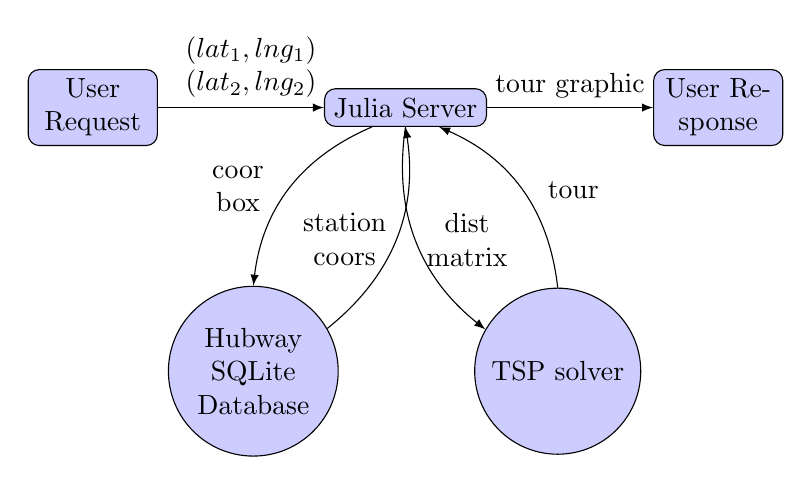
\begin{tikzpicture}
     \draw<1-> node[rectangle, align=center, rounded corners, draw,fill=blue!20, text width = 4em] (req) {User Request};
        \draw <2-> node[rectangle, align = center, rounded corners, draw, fill=blue!20, right=6em of req] (server) {Julia Server};
        \path<3-> (server) ++(-120:11em) node[circle, draw, align=center, fill=blue!20, text width = 5em,inner sep = .1em, minimum size= 6em] (database) {Hubway SQLite Database};
        \path<4-> (server) ++(-60:11em) node[circle, draw, align=center, fill=blue!20, text width = 5em, inner sep = .1em, minimum size= 6em] (tsp) {TSP solver};
        \draw <5-> node[rectangle, rounded corners, align=center, draw, fill=blue!20, right= 6em of server, text width = 4em] (resp) {User Response};
        \draw <2-> (req) edge[->,draw,>=latex] node[above, align=center, text width = 4em] {$(lat_1,lng_1)$ $(lat_2,lng_2)$} (server);
        \draw <3-> (server) edge[->,draw,>=latex, bend right] node[left, align=center, text width = 3em] {coor box} (database);
        \draw <3-> (database) edge[->,draw,>=latex, bend right] node[left, align=center, text width = 3em] {station coors} (server);
        \draw <4-> (server) edge[->,draw,>=latex, bend right] node[right, align=center, text width = 3em] {dist matrix} (tsp);
        \draw <4-> (tsp) edge[->,draw,>=latex, bend right] node[right, align=center, text width = 3em] {tour} (server);
        \draw <5-> (server) edge[->,draw,>=latex] node[above] {tour graphic} (resp);
      \end{tikzpicture}

\end{frame}

\begin{frame}
  \frametitle{Last Time}
  \begin{itemize}
  \item The internet\pause
  \item Databases\pause
  \item Name Service\pause
  \item {\bf Stations Service:} $(lat,lng)$ for all hubway stations in a box
  \end{itemize}

\end{frame}

\begin{frame}
  \frametitle{Today}
  \begin{itemize}
  \item MIP callbacks\pause
  \item TSP\pause
  \item {\bf Convert Stations Service to TSP Service}\pause
  \item Deploying MIP solvers in the real world
  \end{itemize}

\end{frame}


\section{MIP Callbacks}
\subsection{}

\begin{frame}
  \frametitle{What is a MIP Callback?}

  \emph{Callbacks interrupt the MIP solver to run custom code.}\pause

  \vspace{2em}
  Things you can do with MIP callbacks:
  \begin{itemize}
  \item Add constraints to the problem\pause
  \item Suggest new integer solutions\pause
  \item Control branching \& node selection\pause
  \item Log {\bf anything} about solver progress for offline analysis
  \end{itemize}

\end{frame}
\begin{frame}
  \frametitle{How does a MIP solver work anyway?}
  \begin{small}
  \begin{columns}
    \begin{column}{.5\linewidth}
      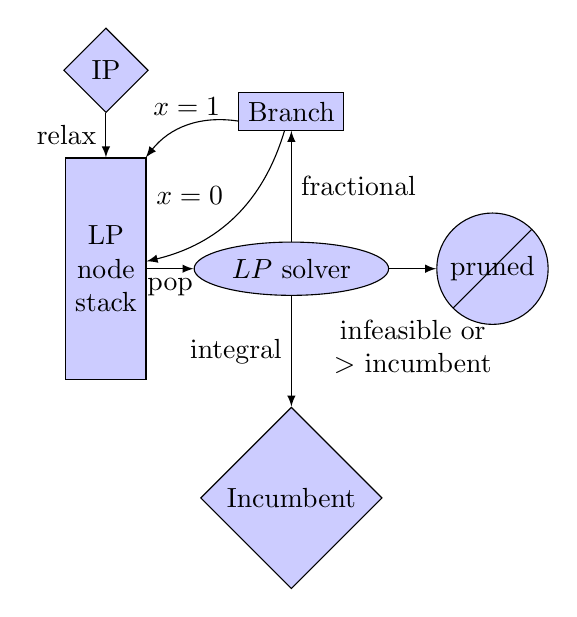
\begin{tikzpicture}
        \draw<1-> node[diamond,draw,fill=blue!20] (IP) {IP};
        \draw <1-> node[rectangle, minimum height = 8em, align=center, color=white, below=1.6em of IP] (hiddenStack) {stack};
        \draw <2-> node[rectangle,draw,fill=blue!20, minimum height = 8em, align=center, below=1.6em of IP] (stack) {LP\\node\\stack};
        \draw <1-> node[ellipse, color= white,right=1.7em of hiddenStack] (hiddenLPsolver) {$LP$ solver};
        \draw <3->node[ellipse, draw,fill=blue!20,regular polygon sides=5, right=1.7em of stack] (LPsolver) {$LP$ solver};
        \draw<4-> node[forbidden sign,draw,fill=blue!20,fill=blue!20, right= 1.7em of LPsolver] (pruned) {pruned};
        \draw<2-> node[diamond, inner sep = .3em, draw,fill=blue!20,below=4em of hiddenLPsolver] (incumbent) {Incumbent};
        \draw <5->node[rectangle,draw,fill=blue!20, above=4em of LPsolver] (branch) {Branch};
        \draw<2-> (IP) edge[->,>=latex] node[left,black] {relax} (stack);
        \draw<3-> (stack) edge[->,>=latex] node[below,black] {pop} (LPsolver);
        \draw<4-> (LPsolver) edge[->,>=latex] node[below=1.5em,black,align=center] {infeasible or\\ $>$ incumbent} (pruned);
        \draw<5-> (LPsolver) edge[->,>=latex] node[right,black] {fractional} (branch);
        \draw<5-> (branch) edge[->,>=latex,bend right] node[above] {$x=1$} (stack);
        \draw<5-> (branch) edge[->,>=latex,bend left] node[above left=.1em] {$x=0$} (stack);
        \draw<6-> (LPsolver) edge[->,>=latex] node[left] {integral} (incumbent);
      \end{tikzpicture}
    \end{column}
    \begin{column}{.55\linewidth}
      \pause
      \begin{algorithm}[H]
        % \KwData{An IP}        
        Add LP relaxation to node stack\;
        Incumbent $=$ \texttt{null}\;\pause
        \While{node stack not empty}{
          Pop LP from node stack \& solve\;\pause
          \uIf{Infeasible or $>$ incumbent}{Discard node}\pause
          \uElseIf{Fractional}{Branch on fractional variable}\pause
          \Else{Set incumbent to solution}
        }
        \KwRet{incumbent}
      \end{algorithm}              
    \end{column}
  \end{columns}      
  \end{small}
\end{frame}
\begin{frame}
  \frametitle{The Lazy Constraint Callback}
  Add the ``lazy'' constraints only once they have been violated by an integer solution.
  
  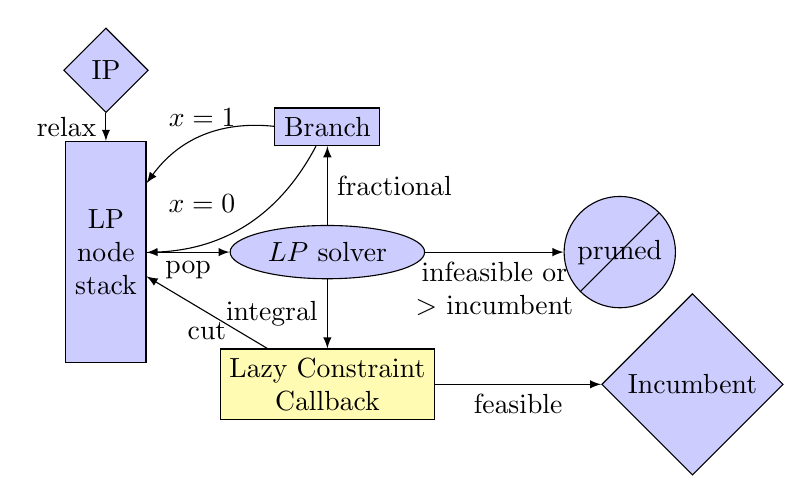
\begin{tikzpicture}
    \draw<1-> node[diamond,draw,fill=blue!20] (IP) {IP};
    \draw <1-> node[rectangle,draw,fill=blue!20, minimum height = 8em, align=center, below=1em of IP] (stack) {LP\\node\\stack};
    \draw <1->node[ellipse, draw,fill=blue!20,regular polygon sides=5, right=3em of stack] (LPsolver) {$LP$ solver};
    \draw<1-> node[forbidden sign,draw,fill=blue!20,fill=blue!20, right= 5em of LPsolver] (pruned) {pruned};
    \draw<1-> node[rectangle, draw, fill=yellow!30, below = 2.5em of LPsolver, align=center] (lazy) {Lazy Constraint\\Callback};
    \draw<1-> node[diamond, inner sep = .3em, draw,fill=blue!20,right=6em of lazy] (incumbent) {Incumbent};
    \draw <1->node[rectangle,draw,fill=blue!20, above=of LPsolver] (branch) {Branch};
    \draw<1-> (IP) edge[->,>=latex] node[left,black] {relax} (stack);
    \draw<1-> (stack) edge[->,>=latex] node[below,black] {pop} (LPsolver);
    \draw<1-> (LPsolver) edge[->,>=latex] node[below,black,align=center] {infeasible or\\ $>$ incumbent} (pruned);
    \draw<1-> (LPsolver) edge[->,>=latex] node[right,black] {fractional} (branch);
    \draw<1-> (branch) edge[->,>=latex,bend right] node[above] {$x=1$} (stack);
    \draw<1-> (branch) edge[->,>=latex,bend left] node[above left=.1em] {$x=0$} (stack);
    \draw<1-> (LPsolver) edge[->,>=latex] node[left] {integral} (lazy);
    \draw<1-> (lazy) edge[->,>=latex] node[below] {feasible} (incumbent);
    \draw<1-> (lazy) edge[->,>=latex] node[below] {cut} (stack);
  \end{tikzpicture}
   
\end{frame}
\begin{frame}
    \frametitle{When to make a family of constraints lazy}
  \begin{columns}
    \begin{column}[t]{.5\linewidth}
      {\bf Good idea when:}
      \begin{itemize}
      \item Family of constraints is large (e.g.\ $n^3$, $2^n$, $|\mathbb R|$)
      \item Integer solutions quickly \emph{separated}
      \item Most constraints not violated
      \end{itemize}
    \end{column}\pause
    \begin{column}[t]{.5\linewidth}
      {\bf Problems:}
      \begin{itemize}
      \item Hard to find an integer solution
      \item Best bound improves slowly if many lazy constraints needed
      \end{itemize}
    \end{column}
  \end{columns}
  

\end{frame}

\begin{frame}
  \frametitle{Lazy Constraints in Julia}
  \begin{columns}
    \begin{column}[t]{.3\linewidth}
      {\bf Simple Lazy IP:}
      \begin{align*}
        &\max&x_1 + 2 x_2\\
        &\text{lazy:}& x_1 + x_2 &\leq 1\\
        &&x_1,x_2&\in \{0,1\}
      \end{align*}
    \end{column}
    \begin{column}[t]{.7\linewidth}
      {\bf Julia Solution:}
      \pause
      \begin{footnotesize}
      \begin{Verbatim}[commandchars=\\\{\}]
\PY{n}{m} \PY{o}{=} \PY{n}{Model}\PY{p}{(}\PY{n}{solver}\PY{o}{=}\PY{n}{GurobiSolver}\PY{p}{(}\PY{n}{LazyConstraints}\PY{o}{=}\PY{l+m+mi}{1}\PY{p}{)}\PY{p}{)}
\PY{p}{@}\PY{n}{defVar}\PY{p}{(}\PY{n}{m}\PY{p}{,}\PY{n}{x}\PY{p}{[}\PY{l+m+mi}{1}\PY{p}{:}\PY{l+m+mi}{2}\PY{p}{]}\PY{p}{,}\PY{n}{Bin}\PY{p}{)}
\PY{p}{@}\PY{n}{setObjective}\PY{p}{(}\PY{n}{m}\PY{p}{,}\PY{n}{Max}\PY{p}{,} \PY{n}{x}\PY{p}{[}\PY{l+m+mi}{1}\PY{p}{]} \PY{o}{+} \PY{l+m+mi}{2}\PY{o}{*}\PY{n}{x}\PY{p}{[}\PY{l+m+mi}{2}\PY{p}{]}\PY{p}{)}
\PY{k}{function}\PY{n+nf}{ }\PY{n+nf}{lazy}\PY{p}{(}\PY{n}{cb}\PY{p}{)}
    \PY{n}{xVal} \PY{o}{=} \PY{n}{getValue}\PY{p}{(}\PY{n}{x}\PY{p}{)}
    \PY{k}{if} \PY{n}{xVal}\PY{p}{[}\PY{l+m+mi}{1}\PY{p}{]} \PY{o}{+} \PY{n}{xVal}\PY{p}{[}\PY{l+m+mi}{2}\PY{p}{]} \PY{o}{\PYZgt{}} \PY{l+m+mi}{1} \PY{o}{+} \PY{l+m+mf}{1e\PYZhy{}4}
        \PY{p}{@}\PY{n}{addLazyConstraint}\PY{p}{(}\PY{n}{cb}\PY{p}{,} \PY{n}{x}\PY{p}{[}\PY{l+m+mi}{1}\PY{p}{]} \PY{o}{+} \PY{n}{x}\PY{p}{[}\PY{l+m+mi}{2}\PY{p}{]} \PY{o}{\PYZlt{}=} \PY{l+m+mi}{1}\PY{p}{)}
    \PY{k}{end}
\PY{k}{end}
\PY{n}{setlazycallback}\PY{p}{(}\PY{n}{m}\PY{p}{,}\PY{n}{lazy}\PY{p}{)}
\PY{n}{solve}\PY{p}{(}\PY{n}{m}\PY{p}{)}
\end{Verbatim}
        
      \end{footnotesize}
    \end{column}
  \end{columns}

\end{frame}

\begin{frame}
  \frametitle{Exercise: the feasible circle}
    {\bf Input:} radius $r$, direction $\mathbf c = (c_1,c_2)$\\
    {\bf Goal:} maximize $\mathbf c \cdot \mathbf x$ on integer inside radius $r$ circle.\pause
    \begin{columns}
      \begin{column}{.5\linewidth}
        \begin{align*}
          &\max& \mathbf c \mathbf x\\
          &\text{subject to:}& \|\mathbf x\|_2 &\leq r\\
          &&\mathbf x &\in \mathbb Z_2
        \end{align*}
      \end{column}
      \begin{column}{.5\linewidth}
        $r = 5$, $\mathbf c = (2,1)$
        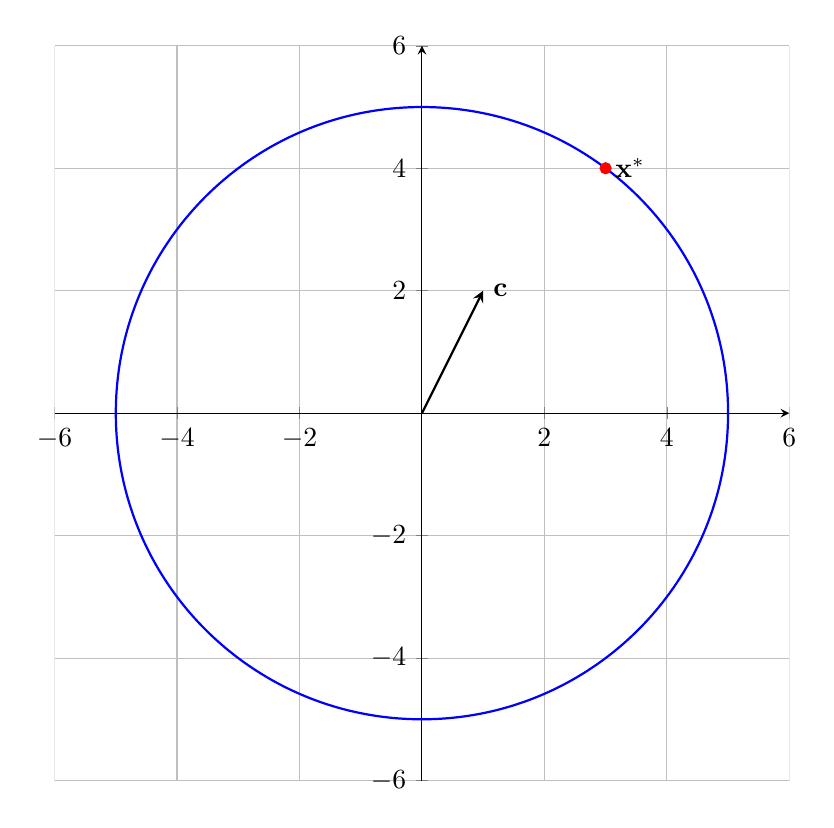
\begin{tikzpicture}
          \begin{axis}[height = .9\linewidth, width = .9\linewidth,
            xmin=-6,   xmax=6, ymin=-6, ymax=6,
            axis lines = center, grid = major]
            \draw[blue, thick] \pgfextra{\pgfpathellipse{\pgfplotspointaxisxy{0}{0}}
              {\pgfplotspointaxisdirectionxy{5}{0}}
              {\pgfplotspointaxisdirectionxy{0}{5}}          
            };
            \addplot [-stealth, thick] plot coordinates {(0,0) (1,2)} node[right] {$\mathbf c$};
            \addplot [red,mark=*, only marks] coordinates {(3,4)} node[right,black] {$\mathbf x^*$};
          \end{axis}
        \end{tikzpicture}\\
        $\mathbf x^* = (3,4)$
      \end{column}
    \end{columns}
\end{frame}

\begin{frame}
  \frametitle{Solving the feasible circle with Lazy Constraint Callbacks}
  \begin{columns}
    \begin{column}[t]{.4\linewidth}
        {\bf Lazy Formulation:}
        \begin{align*}
          &\max& \mathbf c \cdot \mathbf x\\
          &\text{s.t.} &-r \leq x_i & \leq r& i= 1,2\\
          &\text{lazy:}& \mathbf d \cdot \mathbf x &\leq r & \forall \|\mathbf d\|_2 = 1 \\
          &&\mathbf x &\in \mathbb Z_2
        \end{align*}\pause
        \begin{center}
          
         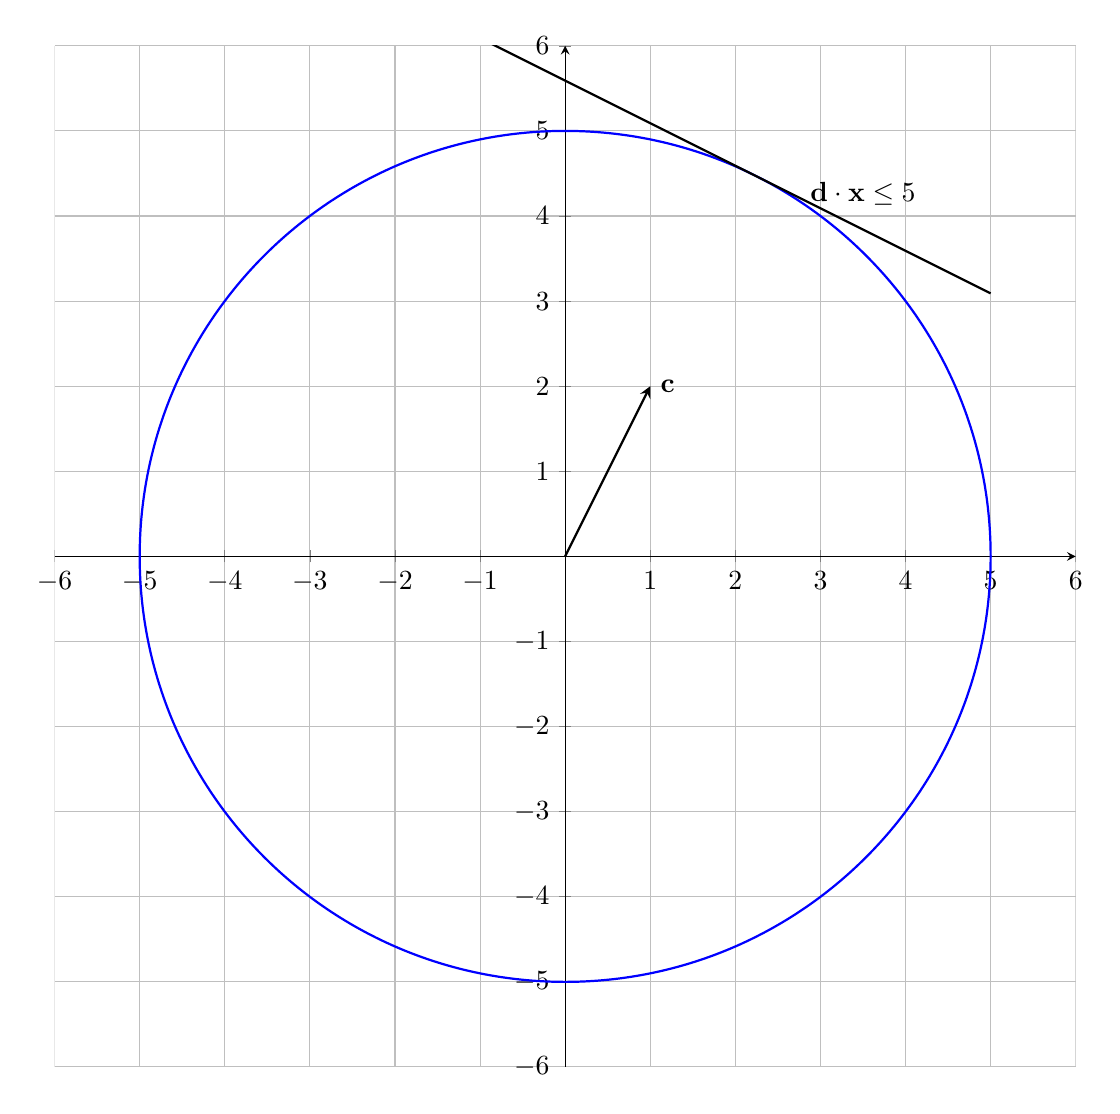
\begin{tikzpicture}
          \begin{axis}[height = 1.2\linewidth, width = 1.2\linewidth,
            xmin=-6,   xmax=6, ymin=-6, ymax=6,
            axis lines = center, grid = major]
            \draw[blue, thick] \pgfextra{\pgfpathellipse{\pgfplotspointaxisxy{0}{0}}
              {\pgfplotspointaxisdirectionxy{5}{0}}
              {\pgfplotspointaxisdirectionxy{0}{5}}          
            };
            \addplot [-stealth, thick] plot coordinates {(0,0) (1,2)} node[right] {$\mathbf c$};
            \addplot [thick,black] {5/0.894427 - 0.447214*x/0.894427} node[above=.5em, pos=.85] {$\mathbf d \cdot \mathbf x \leq 5$};
            %\addplot [domain=-5:5,pattern=north east lines] {5/0.894427 - 0.447214*x/0.894427} |- {(5,-5), (-5,-5)} \closedcycle;
          \end{axis}
        \end{tikzpicture}\\
        $\mathbf d = \frac{1}{\|c\|} \mathbf c$.
        \end{center}
        
    \end{column}\pause
    \begin{column}[t]{.6\linewidth}      
  {\bf Implementing Lazy Constraints:}
  \begin{itemize}
  \item Uncountably many! \pause
  \item If $\|\mathbf x\|_2 > r$, take $\mathbf d = \frac{1}{\|\mathbf x\|_2}\mathbf x$, as 
    \begin{align*}
      \mathbf d \cdot \mathbf x =  \frac{1}{\|x\|_2}\mathbf x\cdot \mathbf x = \|\mathbf x\|_2 > r
    \end{align*}\pause
  \item Psuedo code:
    \begin{algorithm}[H]
      \If{$\|\mathbf x\|_2 > r$}{
        $\mathbf d = \frac{1}{\|\mathbf x\|_2} \mathbf x$\;
        add lazy constraint $\mathbf d \cdot \mathbf x \leq r$\;
      }
    \end{algorithm}
    \end{itemize}
    \end{column}
  \end{columns}
  
\end{frame}

\begin{frame}
  \frametitle{Lazy constraints vs.\ Lazy constraint callbacks} Some
  solvers support lazy constraints without callbacks.  However, they
  have the following limitations:
  \begin{itemize}
  \item All constraints must be generated at start
  \item Each constraint is checked manually against integer solutions.
  \end{itemize}
  Wouldn't work for the ``feasible circle.''
\end{frame}

\begin{frame}
  \frametitle{User Cut Callback}

   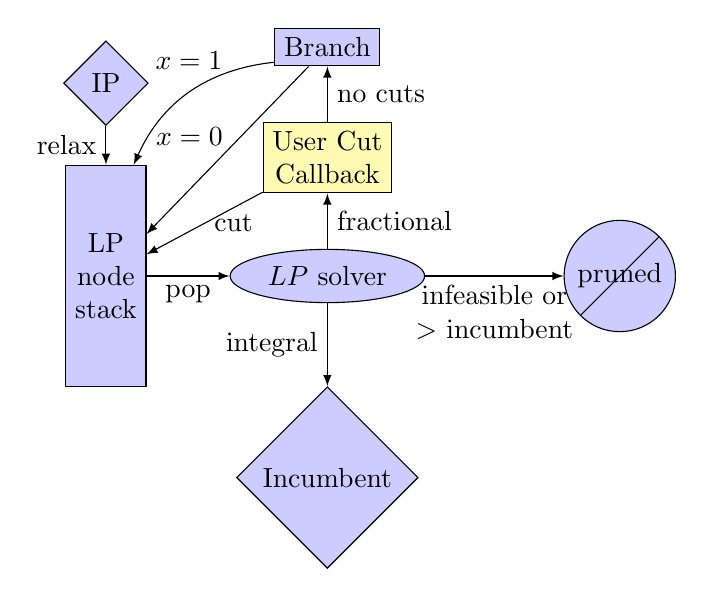
\begin{tikzpicture}
    \draw<1-> node[diamond,draw,fill=blue!20] (IP) {IP};
    \draw <1-> node[rectangle,draw,fill=blue!20, minimum height = 8em, align=center, below=1.4em of IP] (stack) {LP\\node\\stack};
    \draw <1->node[ellipse, draw,fill=blue!20,regular polygon sides=5, right=3em of stack] (LPsolver) {$LP$ solver};
    \draw<1-> node[forbidden sign,draw,fill=blue!20,fill=blue!20, right= 5em of LPsolver] (pruned) {pruned};
    \draw<1-> node[diamond, inner sep = .3em, draw,fill=blue!20,below=3em of LPsolver] (incumbent) {Incumbent};
    \draw<1-> node[rectangle, draw, fill=yellow!30, above = 2em of LPsolver, align=center] (user) {User Cut\\Callback};
    \draw <1->node[rectangle,draw,fill=blue!20, above=2em of user] (branch) {Branch};
    \draw<1-> (IP) edge[->,>=latex] node[left,black] {relax} (stack);
    \draw<1-> (stack) edge[->,>=latex] node[below,black] {pop} (LPsolver);
    \draw<1-> (LPsolver) edge[->,>=latex] node[below,black,align=center] {infeasible or\\ $>$ incumbent} (pruned);
    \draw<1-> (LPsolver) edge[->,>=latex] node[right,black] {fractional} (user);
    \draw<1-> (user) edge[->,>=latex] node[right,black] {no cuts} (branch);
    \draw<1-> (user) edge[->,>=latex] node[right,black] {cut} (stack);
    \draw<1-> (branch) edge[->,>=latex,bend right] node[above=.5em] {$x=1$} (stack);
    \draw<1-> (branch) edge[->,>=latex] node[above left=-.25em] {$x=0$} (stack);
    \draw<1-> (LPsolver) edge[->,>=latex] node[left] {integral} (incumbent);
  \end{tikzpicture}
\end{frame}


\begin{frame}
  \frametitle{Heuristic Callback}
   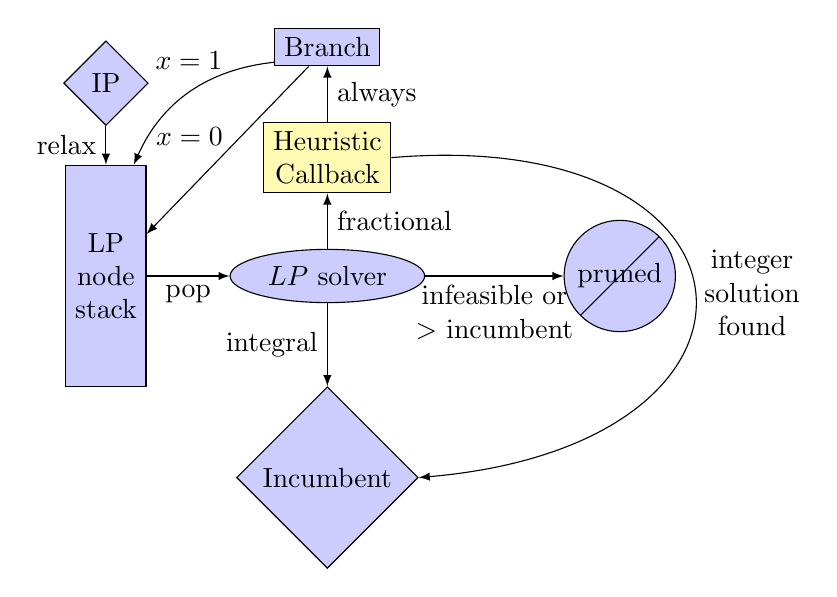
\begin{tikzpicture}
    \draw<1-> node[diamond,draw,fill=blue!20] (IP) {IP};
    \draw <1-> node[rectangle,draw,fill=blue!20, minimum height = 8em, align=center, below=1.4em of IP] (stack) {LP\\node\\stack};
    \draw <1->node[ellipse, draw,fill=blue!20,regular polygon sides=5, right=3em of stack] (LPsolver) {$LP$ solver};
    \draw<1-> node[forbidden sign,draw,fill=blue!20,fill=blue!20, right= 5em of LPsolver] (pruned) {pruned};
    \draw<1-> node[diamond, inner sep = .3em, draw,fill=blue!20,below=3em of LPsolver] (incumbent) {Incumbent};
    \draw<1-> node[rectangle, draw, fill=yellow!30, above = 2em of LPsolver, align=center] (user) {Heuristic\\Callback};
    \draw <1->node[rectangle,draw,fill=blue!20, above=2em of user] (branch) {Branch};
    \draw<1-> (IP) edge[->,>=latex] node[left,black] {relax} (stack);
    \draw<1-> (stack) edge[->,>=latex] node[below,black] {pop} (LPsolver);
    \draw<1-> (LPsolver) edge[->,>=latex] node[below,black,align=center] {infeasible or\\ $>$ incumbent} (pruned);
    \draw<1-> (LPsolver) edge[->,>=latex] node[right,black] {fractional} (user);
    \draw<1-> (user) edge[->,>=latex,bend left = 90, distance = 14em] node[right,black,align=center] {integer\\solution\\found} (incumbent);
    \draw<1-> (user) edge[->,>=latex] node[right,black] {always} (branch);
    \draw<1-> (branch) edge[->,>=latex,bend right] node[above=.5em] {$x=1$} (stack);
    \draw<1-> (branch) edge[->,>=latex] node[above left=-.25em] {$x=0$} (stack);
    \draw<1-> (LPsolver) edge[->,>=latex] node[left] {integral} (incumbent);
  \end{tikzpicture}
\end{frame}

\begin{frame}
  \frametitle{Other callbacks}
  \begin{itemize}
  \item {\bf Incumbent Callback:} optionally reject solutions, improvement heuristics
  \item {\bf Branching Callback:} select variable/constraint to branch on
  \item {\bf Node Selection Callback:} select node from node stack
  \end{itemize}
\end{frame}






\section{TSP}
\subsection{}

\begin{frame}
  \frametitle{The Traveling Salesman Problem}
  \begin{columns}
    \begin{column}{.45\linewidth}
      {\bf The TSP:}
      \begin{itemize}
      \item $n$ cities
      \item $c_{ij}$ cost between cities
        \begin{itemize}
        \item (Euclidean distance)
        \end{itemize}
      \item Visit each city once
      \item Minimize total cost
      \end{itemize}      
    \end{column}
    \begin{column}{.6\linewidth}
      \begin{tiny}
              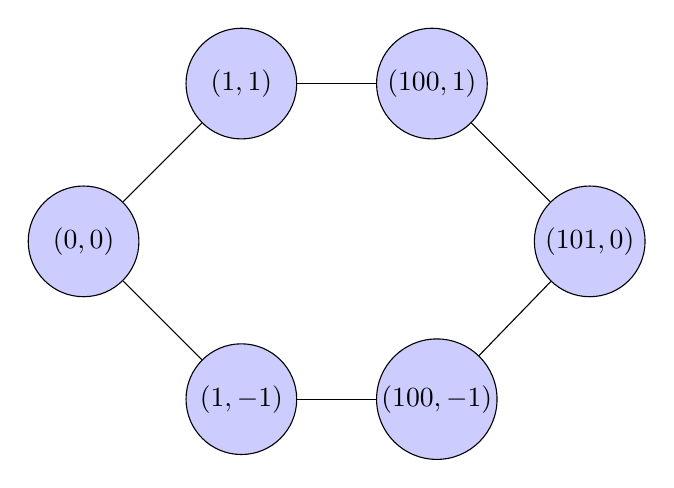
\begin{tikzpicture}
        \draw node[draw, inner sep = .1em, minimum size = 4em, fill=blue!20,circle] (a1) {$(0,0)$};
        \draw node[draw, inner sep = .1em, minimum size = 4em,fill=blue!20,circle, above right = of a1] (a2) {$(1,1)$};
        \draw node[draw, inner sep = .1em, minimum size = 4em,fill=blue!20,circle, below right = of a1] (a3) {$(1,-1)$};
        \draw node[draw, inner sep = .1em, minimum size = 4em,fill=blue!20,circle,right = of a2] (a4) {$(100,1)$};
        \draw node[draw, inner sep = .1em, minimum size = 4em,fill=blue!20,circle, right = of a3] (a5) {$(100,-1)$};
        \draw node[draw, inner sep = .1em, minimum size = 4em,fill=blue!20,circle, below right = of a4] (a6) {$(101,0)$};
        \draw (a1) edge[-,>=latex] (a2);
        \draw (a2) edge[-,>=latex] (a4);
        \draw (a4) edge[-,>=latex] (a6);
        \draw (a6) edge[-,>=latex] (a5);
        \draw (a5) edge[-,>=latex] (a3);
        \draw (a3) edge[-,>=latex] (a1);
      \end{tikzpicture}      
    \end{tiny}
    Optimal tour, geometric $c_{ij}$.
    \end{column}
  \end{columns}
\end{frame}
\begin{frame}
  \frametitle{IP for TSP}
  \begin{itemize}
  \item Graph $G = (V,E)$
  \item $\delta(v) = $ edges incident to $v$
  \item For $S \subset V$, $\delta(S) = $ edges with {\bf one} endpoint in $S$
  \end{itemize}\pause
  \begin{columns}
    \begin{column}{.45\linewidth}
        \begin{align*}
    &\min&\sum_{e \in E} c_e x_e\\
    &\text{s.t.}&\sum_{e \in \delta(v)} x_e &= 2 & \forall v &\in V\\
    &&\sum_{e \in \delta(S)} x_e &\geq 2 & \forall S &\subset V,\\
    &&&&S &\neq \emptyset, V\\
    &&x_e \in \{0,1\}
  \end{align*}
  \pause
    \end{column}
      \begin{column}{.6\linewidth}
      \begin{tiny}
        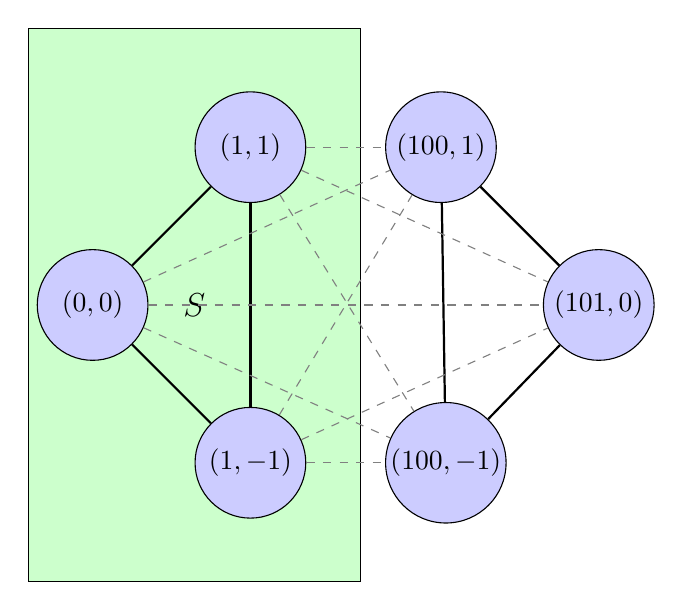
\begin{tikzpicture}
          \draw node[] (start) {};
          \draw node[draw, rectangle, minimum width = 12em,  minimum height = 20em, fill=green!20] {\large $S$};
          \draw node[draw, inner sep = .1em, minimum size = 4em, fill=blue!20,circle, left = 1.3em of start] (a1) {$(0,0)$};          
        \draw node[draw, inner sep = .1em, minimum size = 4em,fill=blue!20,circle, above right = of a1] (a2) {$(1,1)$};
        \draw node[draw, inner sep = .1em, minimum size = 4em,fill=blue!20,circle, below right = of a1] (a3) {$(1,-1)$};
        \draw node[draw, inner sep = .1em, minimum size = 4em,fill=blue!20,circle,right = of a2] (a4) {$(100,1)$};
        \draw node[draw, inner sep = .1em, minimum size = 4em,fill=blue!20,circle, right = of a3] (a5) {$(100,-1)$};
        \draw node[draw, inner sep = .1em, minimum size = 4em,fill=blue!20,circle, below right = of a4] (a6) {$(101,0)$};
        \draw (a1) edge[thick,-,>=latex] (a2);
        \draw (a2) edge[thick,-,>=latex] (a3);
        \draw (a4) edge[thick,-,>=latex] (a6);
        \draw (a6) edge[thick,-,>=latex] (a5);
        \draw (a5) edge[thick,-,>=latex] (a4);
        \draw (a3) edge[thick,-,>=latex] (a1);

        \draw (a1) edge[dashed, color = gray] (a4);
        \draw (a1) edge[dashed, color = gray] (a5);
        \draw (a1) edge[dashed, color = gray] (a6);
        \draw (a2) edge[dashed, color = gray] (a4);
        \draw (a2) edge[dashed, color = gray] (a5);
        \draw (a2) edge[dashed, color = gray] (a6);
        \draw (a3) edge[dashed, color = gray] (a4);
        \draw (a3) edge[dashed, color = gray] (a5);
        \draw (a3) edge[dashed, color = gray] (a6);
      \end{tikzpicture}      
    \end{tiny}
    A violated cutset constraint
    \end{column}
  \end{columns}
\end{frame}

\begin{frame}
  \frametitle{Exercise: Solving TSP in Julia w/o cutset constraints}
  {\bf Input:} a symmetric 2d matrix $c_{ij}$ with $c_{ii} = 0$\\
  {\bf Output:} the optimal cost, and an array with the city indices in order\\
  {\bf Step 1:} Ignore the cutset constraints, make sure it works.
  \begin{itemize}
  \item Create variables $x_{ij}$ for $i = 1,\ldots,n$, $j = 1,\ldots,n$
  \item Add constraints
    \begin{align*}
      x_{ii} &= 0\\
      x_{ij} &= x_{ji}\\
    \end{align*}
  \item Add degree = 2 constraints \& objective
  \item Use {\tt extractCycle} to get the optimal tour when you are done
  \end{itemize}
\end{frame}
\begin{frame}
  \frametitle{Exercise: Check your work}
  \begin{itemize}
  \item 3 cities (in {\tt testTspSolver.jl})
  \item 6 cities with subtours (in {\tt testTspSolver.jl})
  \item Try {\tt plotTour}
  \end{itemize}
\end{frame}

\begin{frame}
  \frametitle{Exercise: Add cutset constraints with lazy constraints}
  Don't check each of $2^V-2$ cutsets! Use \emph{separation}!\pause
  \begin{itemize}
  \item Degree constraints $\Rightarrow$ integer solution degree two graph\pause
  \item Degree two graphs are a collection of cycles\pause
  \item Each cycle is a violated cutset, $S =$ nodes in cycle\pause
  \item Use {\tt connectedComponents} to get a list of cycles\pause
  \item If $k > 1$ cycles, add cutset constraint for first $k-1$ cycles\pause
  \item Check your work on 6 cities
  \item Try a larger instance from TSPLIB (in {\tt tsplib.jl})
  \end{itemize}
\end{frame}

\begin{frame}
  \frametitle{Aside: the TSP and separation}

  The \emph{separation problem} for a polyhedron $P$:
  \begin{itemize}
  \item Given $\mathbf x$ show $\mathbf x \in P$, or find a violated constraint
  \end{itemize}\pause
  For lazy constraints, we assumed in addition that $\mathbf x$ was integer, a \emph{much easier} problem!\\\vspace{2em}
  
  Use the separation problem for \emph{user cut callbacks}.\\\vspace{2em}

  For TSP, the separation by $n$ Max-Flow Min-Cut
  computations.\\\vspace{2em}

  Challenge: use Julia (make $n$ LPs in each callback)!

\end{frame}
\begin{frame}
  \frametitle{Aside: more callbacks for TSP}

  Easy {\bf heuristic callback}:
  \begin{itemize}
  \item Sort edges by LP relaxation value
  \item For each edge, add if it does not make a cycle
  \end{itemize}\pause
  {\bf Two-Opt:} given an integer TSP solution:
  \begin{itemize}
  \item Find a better solution by changing at most two edges
  \item Repeat until no improvement
  \end{itemize}\pause
  {\bf Incumbent callback + heuristic callback + two-opt}:
  \begin{itemize}
  \item Use incumbent callback to grab integer solutions
  \item Run two-opt
  \item If solution improves, add with heuristic callback
  \end{itemize}  

\end{frame}




\section{TSPaaS}
\subsection{}

\begin{frame}
  \frametitle{Software-as-a-Service (SaaS)}
  
  %\begin{columns}
    %\begin{column}{.5\linewidth}
      Sending a solver is hard
      \begin{itemize}
      \item Licenses
      \item Compiling
      \item Data/Databases
      \item One time revenue
      \end{itemize}
    %\end{column}
    %\begin{column}{.5\linewidth}
    %  
\includegraphics[width=.8\linewidth]{images/sad_image-0.png}
    %\end{column}
    % \end{columns}\pause
      \pause
  %\begin{columns}
  %  \begin{column}{.5\linewidth}
      Bring problem to the solver!
  %  \end{column}
  %  \begin{column}{.5\linewidth}
  %    
\includegraphics[width=.8\linewidth]{images/wink_image-2.png}
  %  \end{column}
  %\end{columns}
  

\end{frame}
\begin{frame}
  \frametitle{TSP-as-a-Service}
  Code is ready. Lets try it!
  \begin{itemize}
  \item Navigate to {\tt cd winstonWorks}
  \item Run {\tt julia tsp\_service\_winston.jl}
  \item Wait for terminal output {\tt Listening on 8000...}
  \item Go to\\
    \begin{footnotesize}
      \url{http://localhost:8000/stationservice/42.3/42.4/-71.2/-71.0}
    \end{footnotesize}
  \end{itemize}\pause
  It worked! Now lets look at {\tt tsp\_service\_winston.jl}
\end{frame}


\section{Deployment}
\subsection{}

\begin{frame}
  \frametitle{Considerations for deploying MIPs}
  \begin{itemize}
  \item Real time or offline MIP solving
  \item Number of simultaneous users
  \item Solver licenses
  \item Reliability/maximum solve time
  \end{itemize}
\end{frame}

\begin{frame}
  \frametitle{Deployment Options}
  \begin{footnotesize}
  \begin{tabular}{lcc}
    \toprule
    Option&Pros&Cons\\
    \midrule
    \begin{minipage}{.2\linewidth}      
      Personal\\
      computer
    \end{minipage}&
    \begin{minipage}{.4\linewidth}
      Easy
    \end{minipage}&
    \begin{minipage}{.4\linewidth}
      Spilled coffee\\
      Two concurrent users\\
      Blackouts\\
      International lag\\
      Data Safety
    \end{minipage}\\
    \midrule
    \begin{minipage}{.2\linewidth}      
      Rent a box
    \end{minipage}&
    \begin{minipage}{.4\linewidth}
      Pretty Easy
    \end{minipage}&
    \begin{minipage}{.4\linewidth}
      Two concurrent users\\
      International lag\\
      Data safety
    \end{minipage}\\
    \midrule
    \begin{minipage}{.2\linewidth}      
      Cloud\\(Amazon/Google)
    \end{minipage}&
    \begin{minipage}{.4\linewidth}
      Scale up for many users\\
      Data safety\\
      Low latency\\
      Monitoring/uptime
    \end{minipage}&
    \begin{minipage}{.4\linewidth}
      Set up time\\
      Learn a system\\
      Can be \$\$
    \end{minipage}\\
    \midrule
    \begin{minipage}{.2\linewidth}
      Gurobi a la cart\\
      (Amazon)\\
      ({\it Solver only})
    \end{minipage}&
    \begin{minipage}{.4\linewidth}
      Pay for what you use\\
      Scale up for many users\\
    \end{minipage}&
    \begin{minipage}{.4\linewidth}
      Can be \$\$\\
      No callbacks
    \end{minipage}\\
    \bottomrule
  \end{tabular}    
  \end{footnotesize}




  
\end{frame}
\end{document}
